\documentclass[a4paper]{article}

% --- Packages ---

\usepackage{a4wide}
\usepackage[utf8]{inputenc}
\usepackage{amsmath}
\usepackage{mathtools}
\usepackage{amssymb}
\usepackage[english]{babel}
\usepackage{mdframed}
\usepackage{systeme,}
\usepackage{lipsum}
\usepackage{relsize}
\usepackage{caption}
\usepackage{tikz}
\usepackage{tikz-3dplot}
\usetikzlibrary{shapes.geometric}
\usepackage{pgfplots}
\usepackage{pgfplotstable}
\pgfplotsset{compat=newest}%1.7}
\usepackage{harpoon}%
\usepackage{graphicx}
\usepackage{wrapfig}
\usepackage{subcaption}
\usepackage{authblk}
\usepackage{float}
\usepackage{listings}
\usepackage{xcolor}
\usepackage{chngcntr}
\usepackage{amsthm}
\usepackage{comment}
\usepackage{commath}
\usepackage{hyperref}%Might remove, adds link to each reference
\usepackage{url}
\usepackage{calligra}
\usepackage{pgf}

% --- Bibtex ---

%\usepackage[backend = biblar,]{bibtex}

%\addbibliografy(ref.bib)

% --- Commands --- 

\newcommand{\w}{\omega}
\newcommand{\trace}{\text{Tr}}
\newcommand{\grad}{\mathbf{\nabla}}
%\newcommand{\crr}{\mathfrak{r}}
\newcommand{\laplace}{\nabla^2}
\newcommand{\newparagraph}{\vspace{.5cm}\noindent}

% --- Math character commands ---

\newcommand{\curl}[1]{\mathbf{\nabla}\times \mathbf{#1}}
\newcommand{\dive}[1]{\mathbf{\nabla}\cdot \mathbf{#1}}
\newcommand{\res}[2]{\text{Res}(#1,#2)}
\newcommand{\fpartial}[2]{\frac{\partial #1}{\partial #2}}
\newcommand{\rot}[3]{\begin{vmatrix}\hat{x}&\hat{y}&\hat{z}\\\partial_x&\partial_y&\partial_z\\#1&#2&#3 \end{vmatrix}}
\newcommand{\average}[1]{\langle #1 \rangle}
\newcommand{\ket}[1]{|#1\rangle}
\newcommand{\bra}[1]{\langle #1|}


%  --- Special character commands ---

\DeclareMathAlphabet{\mathcalligra}{T1}{calligra}{m}{n}
\DeclareFontShape{T1}{calligra}{m}{n}{<->s*[2.2]callig15}{}
\newcommand{\crr}{\mathcalligra{r}\,}
\newcommand{\boldscriptr}{\pmb{\mathcalligra{r}}\,}


\title{INPUT TITLE HERE}
\author{Author : Andreas Evensen}
\date{Date: \today}

% --- Code ---

\definecolor{codegreen}{rgb}{0,0.6,0}
\definecolor{codegray}{rgb}{0.5,0.5,0.5}
\definecolor{codepurple}{rgb}{0.58,0,0.82}
\definecolor{backcolour}{rgb}{0.95,0.95,0.92}

\lstdefinestyle{mystyle}{
    backgroundcolor=\color{backcolour},   
    commentstyle=\color{codegreen},
    keywordstyle=\color{magenta},
    numberstyle=\tiny\color{codegray},
    stringstyle=\color{codepurple},
    basicstyle=\ttfamily\footnotesize,
    breakatwhitespace=false,         
    breaklines=true,                 
    captionpos=b,                    
    keepspaces=true,                 
    numbers=left,                    
    numbersep=5pt,                  
    showspaces=false,                
    showstringspaces=false,
    showtabs=false,                  
    tabsize=2
}

\lstset{style=mystyle}

\begin{document}

\thispagestyle{empty}
\begin{titlepage}
   \begin{center}
       % \vspace*{1cm}
       \huge
       \textbf{Molecular dynamics: Argon Fluid}\\
       \vspace*{1cm}
       \textbf{Course: FK8028}
       \large

       \vspace*{0.5cm}
       \textbf{Author: Andreas Evensen}\\
       \vspace*{.5cm}
       \small
       \vspace*{1.cm}
       \textbf{Submission date: \today}\\
       \vspace*{.5cm}
       \vspace{0.8cm}
     
       \small
       Stockholm University\\
       Computational Physics\\
       Sweden\\
   \end{center}
\end{titlepage}

\pagenumbering{Roman}
\newpage
\pagenumbering{roman}
\setcounter{page}{1}
\newpage
\tableofcontents
\newpage
\pagenumbering{arabic}

\section{Introduction}
In this report, one performed a molecular dynamics simulation with a Lennard-Jones fluid consisting of $N = 125$ argon atoms.
One investigated how the behavior of the simulated system evolved in time.
This was achieved by computing the block-average of the observable quantities of the system, such as the: kinetic energy, potential energy and temperature.
In the following, we will present the method and theory used to compute the block-average, and the results and discussion of the block-average of the observable quantities.

\newparagraph
The simulation ran $T = 300$~ps. Since the system is ergodic, the length of the simulation allowed us to compute the average of the observable quantities of the system as the true average.
\section{Method \& Theory}
In a simulated system one can never achieve true average of any quantity, but in a long enough simulation the average of the same quantity is approaching the true average: this is called ergodicity.
Therefore, we tend to block-analyzis.
Consider an observable $A$ which is computed in a simulation of $N$ iterations.
We can then define so-called blocks which is trying to capture the behavior of the system.
The block-size $k$ is thus a number in-between the value of $1$ and $N$, i.e. the number of elements contained in each block.
The number of blocks is then simply: $n_b = N // k$, where we denoted the floor division. We then define a vector $\mathbf{A}^k$, each element in $\mathbf{A}^k$ is then given by:
\begin{align*}
    A_i^{k} = \frac{1}{k}\sum_{j = 1}^k \mathbf{A}_{k\cdot i + j}.
\end{align*}The variance of the blocks, compared to that of entire data-set is thus given as:
\begin{align*}
    \sigma^2(\mathbf{A}^k) = \frac{1}{n_b}\sum_{i = 1}^{n_b}\left(A_i^k - \bar{A}\right)^2.
\end{align*}The standard deviation of $\bar{A}$ is thus given by:
\begin{align}
    \sigma(\bar{A}) \approx \frac{\sigma(\mathbf{A}^k)}{\sqrt{n_b - 1}}\left(1 \pm \frac{1}{\sqrt{2(n_b - 1)}}\right).\label{eq: standard diviation}
\end{align}The observable $A$ can be any physical quantity measured in the simulation, such as: the kinetic energy $\mathcal{K}$, the potential energy $\mathcal{V}$ and the temperature $T$.
When applying this method, each observable becomes non-correlated, and thus the standard deviation $\sigma(\bar{A})$ can be computed for each observable, which otherwise would not be possible[1].

\newparagraph
Computing the block-average of any observable in the system thus gives us a measurement of how the system behaves, and how long the system have to be simulated until the average is close to the true average.
If the number of blocks is too small, the standard deviation will be large, and the relative error will be large. This is because the system includes has data which is not representative of the true ensemble (the system might not have equilibrated in the first iterations).
For a sufficient number of blocks, the standard deviation will small, and the standard deviation compared to the next increment in number of blocks will be small. This is referred to as the plateau.

\newparagraph
The plateau is the point when the standard deviation $\sigma(\bar{A})$ is constant with creasing number of elements in each block.
At this point, the system has equilibrated and the average of the observable is close to the true average if the system is ergodic.

\newpage
\section{Results \& Discussion}
The simulation ran for a time $T = 300$~ps, the first $30$~ps were discarded as the system was influenced by velocity rescaling and was allowed to equilibrate before sampling.
The block method was implemented with the use of eq \eqref{eq: standard diviation} to compute the $\sigma(\bar{A})$ for the observable quantities of the system.
The results of the block-average of the observable quantities are presented in fig \ref{fig: var_p} -- \ref{fig: var_t}.
\begin{figure}[H]
    \centering
    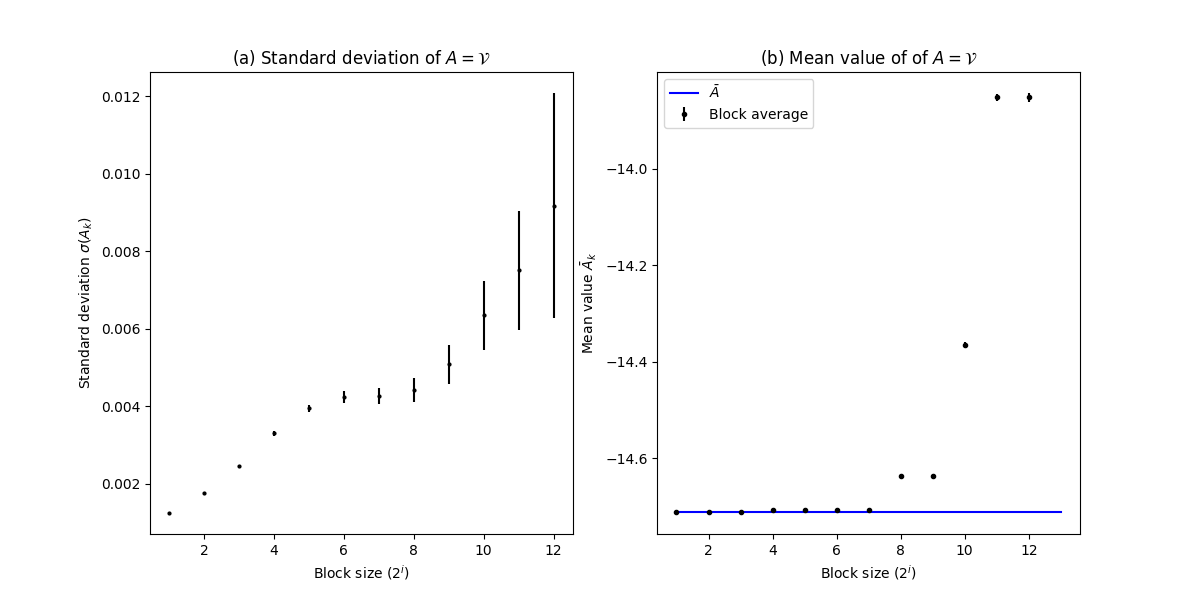
\includegraphics[scale = 0.45]{var_p.png}
    \caption{(a) Standard deviation of $\mathcal{V}$, (b) Mean value as a function of block-size.}
    \label{fig: var_p}
\end{figure}\noindent
In the figure above, fig \ref{fig: var_p}(a), one sees that $\sigma(\mathcal{V})$ is increasing with increasing block-size, until it reaches a so-called plateau.
The uncertainty of the block-average then increases slightly for increasing block-size until it becomes unstable.
In fig \ref{fig: var_p}(b), the mean value of $\mathcal{V}$ is plotted as a function of block-size. The mean value is computed as the mean value of the blocks, and thus it varies with block-size.


\begin{figure}[H]
    \centering
    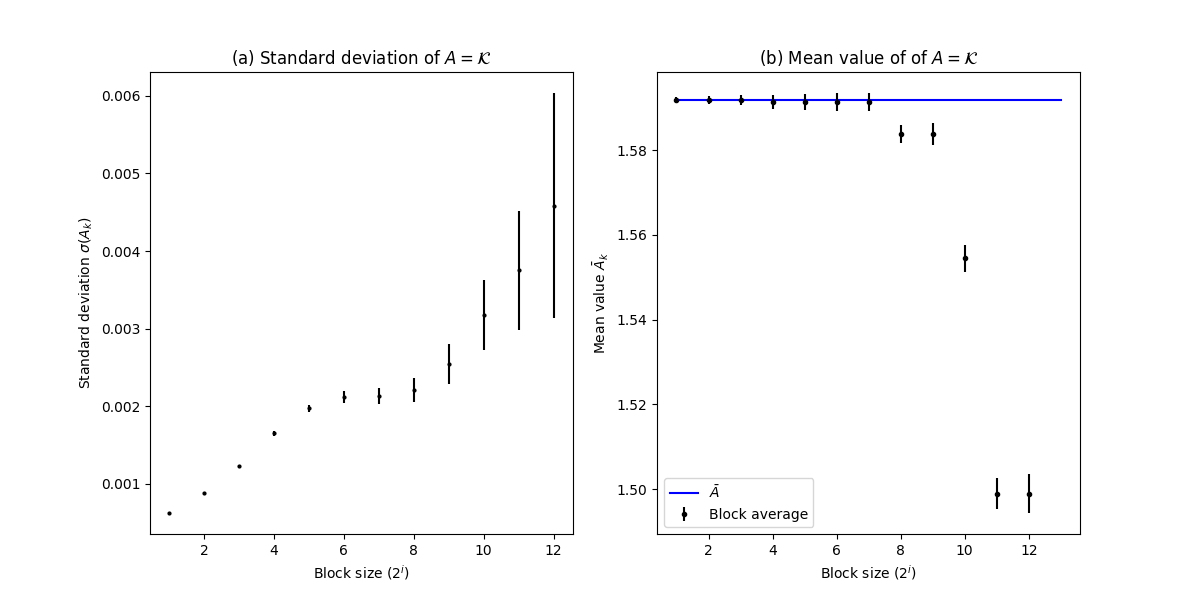
\includegraphics[scale = 0.45]{var_k.png}
    \caption{(a) Standard deviation of $\mathcal{K}$, (b) Mean value as a function of block-size.}
    \label{fig: var_k}
\end{figure}\noindent
Similar to fig \ref{fig: var_p}, the standard deviation of $\mathcal{K}$ is increasing with increasing block-size until it reaches a plateau.
This is seen in fig \ref{fig: var_k}(a); $\sigma(\bar{K})$ is increasing with increasing block-size, and the uncertainty of the block-average then increases slightly for increasing block-size until it becomes unstable.
The mean value of $\mathcal{K}$ is plotted as a function of block-size in fig \ref{fig: var_k}(b), and it is seen that the mean value is computed as the mean value of the blocks, and thus it varies with block-size.

\begin{figure}[H]
    \centering
    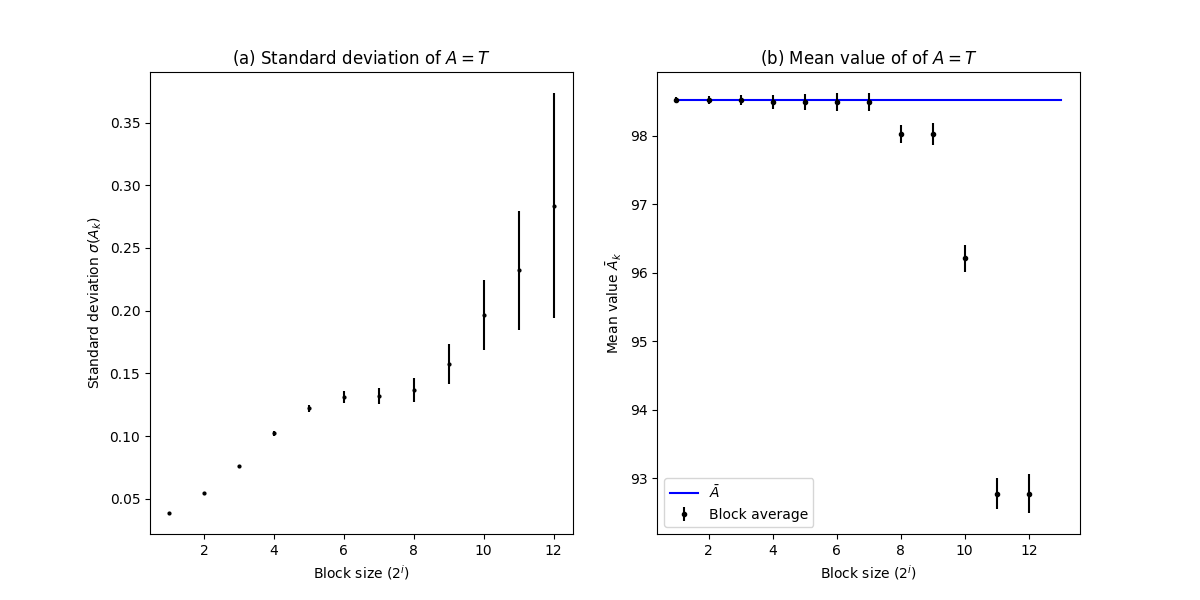
\includegraphics[scale = 0.45]{var_t.png}
    \caption{(a) Standard deviation of $T$, (b) Mean value as a function of block-size.}
    \label{fig: var_t}
\end{figure}\noindent
The temperature $T$ is a function of the kinetic energy, i.e. $T(\mathcal{K})$ and thus $\sigma(T)$ is only different by a constant when comparing the block averaging of $\mathcal{K}$ and $T(\mathcal{K})$.
Hence, it also reaches a plateau at approximately $i = 6$ which corresponds to the block-size being $64$, this is seen in fig \ref{fig: var_t}(a).
The mean value of $T$ is plotted as a function of block-size in fig \ref{fig: var_t}(b), and it is seen that the mean value is computed as the mean value of the blocks, and thus it varies with block-size.

\newparagraph
In fig \ref{fig: var_p}(b) -- \ref{fig: var_t}(b), the mean value of each observable is plotted as a function of the block-size, and it is seen that the mean value is decreasing with increasing block-size.
This is because the system has includes non-equilibrated data in the first iterations, and the block-average is thus not representative of the true ensemble.
The observable mean value, as well as $\sigma(\bar{A})$ and $\frac{\sigma(\bar{A})}{\sqrt{n_b - 1}}$ are presented in table \ref{ref: observables}.
\begin{table}[H]
    \centering
    \caption{Averages of the ensemble of\\ observable for block size $k = 64$.}
    \label{ref: observables}
    \begin{tabular}{|c|c|c|c|}\hline
        &$\mathcal{V}$~(eV) & $\mathcal{K}$~(eV) & $T$~(K)\\\hline
        $\bar{\bar{A}}$& $-14.706$& $1.581$ & $98.489$ \\\hline
        $\sigma(A)$ & $0.00424$ & $0.00212$  & $0.13133$ \\\hline
        $\frac{\sigma(\bar{A})}{\sqrt{n_b - 1}}$ &$0.00015$& $7.3212\cdot 10^{-5}$ & $0.00453$ \\\hline
    \end{tabular}
\end{table}\noindent
The block-size $k = 64$ was determined by comparing the plateaus from figures \ref{fig: var_p}(a)  -- \ref{fig: var_t}(a).
In each figure, the plateau has begun at approximately $i = 6$, which corresponds to the block-size being $64$.
Thus, the block-average is representative of the true ensemble, since the system has equilibrated, and the block-average is close to the true average.

\newparagraph
By comparing block-averages by the averaged value one finds that the system has equilibrated, and that the block-average is representative of the true ensemble: given that we assure ergodicity.
\begin{align}
    \bar{\mathcal{V}} = -14.710 \quad \bar{\mathcal{K}} = 1.5918\quad\bar{T} =98.518. \label{eq: true averages}
\end{align}The difference between the values in table \ref{ref: observables} and the computed averages in eq \eqref{eq: true averages} is small, and thus the block-average is representative of the true ensemble given the prior assumption.

\newpage
\section{Conclusion}
The block-average technique was implemented to compute the standard deviation of the observable quantities of the system.
One saw that $\sigma(\bar{A})$ was increasing with increasing block-size until it reached a plateau.
After this point in became constant, i.e. that the system was invariant to the block-size, which is expected.
This also implies that the block are representative of the true ensemble, and that the system has equilibrated.

\newparagraph
By using the block-average technique, one can compute the standard deviation of the observable quantities of the system, and thus get a measurement of how the system behaves.  
Block-averaging is also a tool to measure how long the system has to be simulated until the average is close to the ensemble average.
If one reaches a plateau the system has equilibrated, and the block-average is representative of the true ensemble.
If no such plateau is reached, the system has not equilibrated and the block-average is not representative of the true ensemble and thus one has to simulate for a longer time.

\newpage
\section*{Reference}

[1]. H. Flyvbjerg and H. G. Petersen. Error estimates on averages of correlated
data. The Journal of Chemical Physics, 91(1):461–466, 1989.


\end{document}
 
